\documentclass{article}

\usepackage{tikz}
\usetikzlibrary{arrows,shapes,automata,petri,positioning,calc,fit}

\tikzset{
    place/.style={
        rectangle,
        thick,
        draw=black,
        fill=gray!50,
        minimum size=6mm,
    },
    lts/.style={
        ellipse,
        draw=black,
        fill=yellow!20,
        minimum size=8mm,
    },
    nfa/.style={
        ellipse,
        draw=black,
        fill=blue!20,
        minimum size=8mm,
    },
    prod/.style={
        ellipse,
        draw=black,
        fill=green!20,
        minimum size=10mm,
    },
    trace/.style={
        draw,
        -,>=stealth',
        semithick,
    },
    trace-point/.style={
        circle,
        draw=black,
        fill=black,
        minimum size=3pt
    },
    every edge/.style={
        draw,
        ->,>=stealth',
        auto,
        semithick
    },
    initial text = {},
    node distance=2.5cm,
    double distance=2pt,
}
\title{PLPDI: Verification Revision Notes}
\author{Sam Barrett}

\begin{document}
\maketitle

\underline{Formal Verification}

This is the application of rigorous, mathematical models to establish the \textbf{correctness} of computerised systems.

\underline{Computer-aided Verification}

Computer-aided verification is simply automated formal verification methods via tools and algorithms etc.

\section{Labelled Transition Systems}

Labelled transition systems are comprised of two parts:

\begin{itemize}
  \item States, representing possible configurations of a systems.
        \begin{itemize}
          \item Values of program variables
          \item Values of registers in a hardware circuit
        \end{itemize}
  \item Transitions, possible ways/routes a system can \textit{evolve}
        \begin{itemize}
          \item Execution of a program statement
          \item Sequential circuit update
        \end{itemize}
\end{itemize}

Formally, they can be defined as a tuple $\texttt{S,Act},\rightarrow , \texttt{I,AP,L} $.
Where:
\begin{itemize}
  \item $\texttt{S} $ is a set of \textbf{states}
  \item $\texttt{Act}$ is a set of \textbf{actions}
  \item $\rightarrow \subseteq \texttt{S}\times \texttt{Act} \times \texttt{S} $ is a \textbf{transition system}
  \item $\texttt{I} \subseteq S$ is a set of \textbf{initial states}
  \item $\texttt{AP} $ is a set of \textbf{atomic propositions}
  \item $\texttt{L:S} \rightarrow 2^{\texttt{AP} } $ is a \textbf{labelling function}
\end{itemize}
\subsection{Example LTS}

\begin{itemize}
  \item $\texttt{S} = \{ \texttt{ready, wait, coffee, beer} \}$
  \item $\texttt{Act} = \{ \texttt{coin, press1, press2, serve}  \} $
\item $\rightarrow = \{ (\texttt{ready, coin, wait} ), \\ (\texttt{wait, press1, coffee} ), \\ (\texttt{wait, press1, beer} ), \\ (\texttt{coffee, serve, ready} ),\\ (\texttt{beer, serve, ready} )\} $
\item $\texttt{I} = \{ \texttt{ready}  \} $
\item $\texttt{AP}  = \{ \texttt{inactive, chosen}  \} $
    \item $\texttt{L(ready)} = \{ \texttt{inactive}  \}, \\ \texttt{L(wait)} = \emptyset , \\ \texttt{L(coffee) = L(beer)} = \{ \texttt{chosen}  \} $
\end{itemize}


\begin{center}
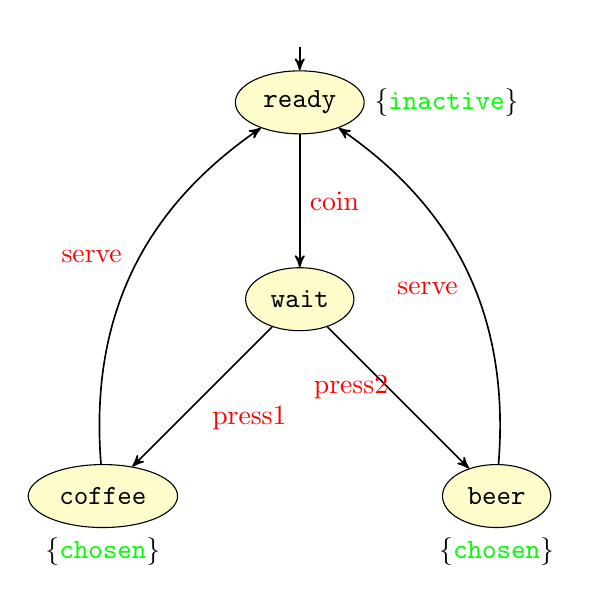
\begin{tikzpicture}
    \node [lts, label=right:{$\{ \color{green}\texttt{inactive} \color{black} \} $}] (S0) {\texttt{ready}};
    \node [above= 3mm of S0] (init) {};

    \node [lts,below of =S0] (wait) {\texttt{wait}};
    \node [lts,below of= wait, left of=wait, label=below:{$\{ \color{green}\texttt{chosen} \color{black} \} $}] (coffee) {\texttt{coffee}};
    \node [lts,below of= wait, right of=wait, label=below:{$\{ \color{green}\texttt{chosen} \color{black} \} $}] (beer) {\texttt{beer}};

    \draw (init) edge (S0);
    \draw (S0) edge node {\color{red}coin} (wait);
    \draw (wait) edge node {\color{red}press1} (coffee);
    \draw (wait) edge node[label=left:{\color{red}press2}] {} (beer);
    \draw (coffee) edge[bend left] node {\color{red}serve} (S0);
    \draw (beer) edge[bend right] node {\color{red}serve} (S0);
    \end{tikzpicture}
\end{center}

\subsection{Labelling \& Finiteness}

LTS states are labelled with \textbf{atomic propositions} $a,b,\ldots \in \texttt{AP} $. They represent facts or observations of the system.

LTS transitions are labelled with actions $\alpha,\beta,\ldots \in \texttt{Act} $ and are used to communicate between \textit{components}

An LTS is said to be \textit{finite} if \texttt{S,Act} and \texttt{AP} are finite. We tend to assume our LTSs are finite.

\subsection{Transitions}

We denote transitions as $s -\alpha\rightarrow s\prime$ if $(s,\alpha,s\prime) \in \rightarrow$

We define the direct successors and predecessors as:
\begin{itemize}
  \item $\texttt{Post}(s,\alpha)= \{ s\prime \in S | s-\alpha\rightarrow s\prime \}  $ and $\texttt{Post}(s) = \cup_{\alpha\in \texttt{Act} } \texttt{Post}(s,\alpha)$
  \item $\texttt{Pre} (s,\alpha) = \{ s\prime \in S | s\prime -\alpha \rightarrow s \} $ and $\texttt{Pre}(s) = \cup_{\alpha\in \texttt{Act} } \texttt{Pre}(s,\alpha) $
\end{itemize}

We say that a state, $s$ is \textbf{terminal} if \texttt{Post}(s) = $\emptyset$, i.e. it has no outgoing transitions. Such states can be used to represent the termination of a program or erroneous or undesired behaviour.


\end{document}
